\documentclass[10pt]{article}
\usepackage[document]{ragged2e}
\usepackage{multicol}
\usepackage[margin=1in]{geometry}
\usepackage{titlesec}
\usepackage{fancyhdr}
\usepackage{graphicx}
\graphicspath{ {./images/} }
\usepackage{bm}
\usepackage{amsmath}
\usepackage{caption}
\captionsetup[subfigure]{justification=centering}
\captionsetup[figure]{justification=centering}
\usepackage{subcaption}
\usepackage{float}

\pagestyle{fancy}
\fancyhf{}
\fancyfoot[R]{Page. \thepage}
\fancypagestyle{plain}{
    \renewcommand{\headrulewidth}{0pt}
    \fancyhf{}
    \fancyfoot[R]{Page. \thepage}
}

\setlength{\parindent}{0em}
\setlength{\parskip}{1em}

\title{MSAI 349 Stock Prediction Project Preliminary Results}
\author{Qingwei Lan}

\begin{document}
\maketitle



\section{Introduction}

Our goal is to develop a trading strategy using stock price and volume data by creating a neural network model to predict stock prices. We will compare our strategies with the already established Buy \& Hold and MACD strategies. Both of these established strategies will be described in detail in the \textbf{Results} section below.


\section{Data Sources}

Throughout this project, we will be using daily stock data taken from Yahoo Finance. For each given day, we have the opening price, closing price, daily high price, daily low price, and trading volume.

We downloaded data for the S\&P 500 index (symbol SPY) for time period Jan. 29, 1993 to Dec. 31, 2020. The data consisted of a total of 7033 observations (trading days). We split our dataset into a training set of size of 5610 and a test set of size 1403. Sample obversations of the dataset is shown in Table \ref{datasample}.

\begin{table}[H]
\centering
\begin{tabular}{| c | c c c c c |} 
\hline
Date & Open & High & Low & Close & Volume \\
\hline
1993-01-29 & 25.735672  & 25.735672  & 25.607634  & 25.717381  & 1003200 \\
1993-02-01 & 25.735661  & 25.900282  & 25.735661  & 25.900282  & 480500 \\
1993-02-02 & 25.882007  & 25.973463  & 25.827133  & 25.955172  & 201300 \\
1993-02-03 & 25.991755  & 26.247831  & 25.973463  & 26.229540  & 529400 \\ 
1993-02-04 & 26.320994  & 26.394158  & 26.028335  & 26.339285  & 531500 \\
... & ... & ... & ... & ... & ... \\
2020-12-24 & 364.514223 & 365.455032 & 363.890351 & 365.425323 & 26457900 \\
2020-12-28 & 368.138779 & 368.980551 & 367.475286 & 368.564636 & 39000400 \\
2020-12-29 & 370.188752 & 370.376914 & 367.237609 & 367.861511 & 53680500 \\
2020-12-30 & 368.732999 & 369.485646 & 367.970469 & 368.386383 & 49455300 \\
2020-12-31 & 368.178394 & 371.030499 & 367.633734 & 370.258057 & 78520700 \\
\hline
\end{tabular}
\caption{Sample stock data for the S\&P 500 index}
\label{datasample}
\end{table}


Since this is a time-series dataset, we will omit the descriptive statistics such as mean and standard deviation. Instead we include a plot of the price of the S\&P 500 index throughout the years in Figure \ref{sp500price}.

\begin{figure}[H]
\centering
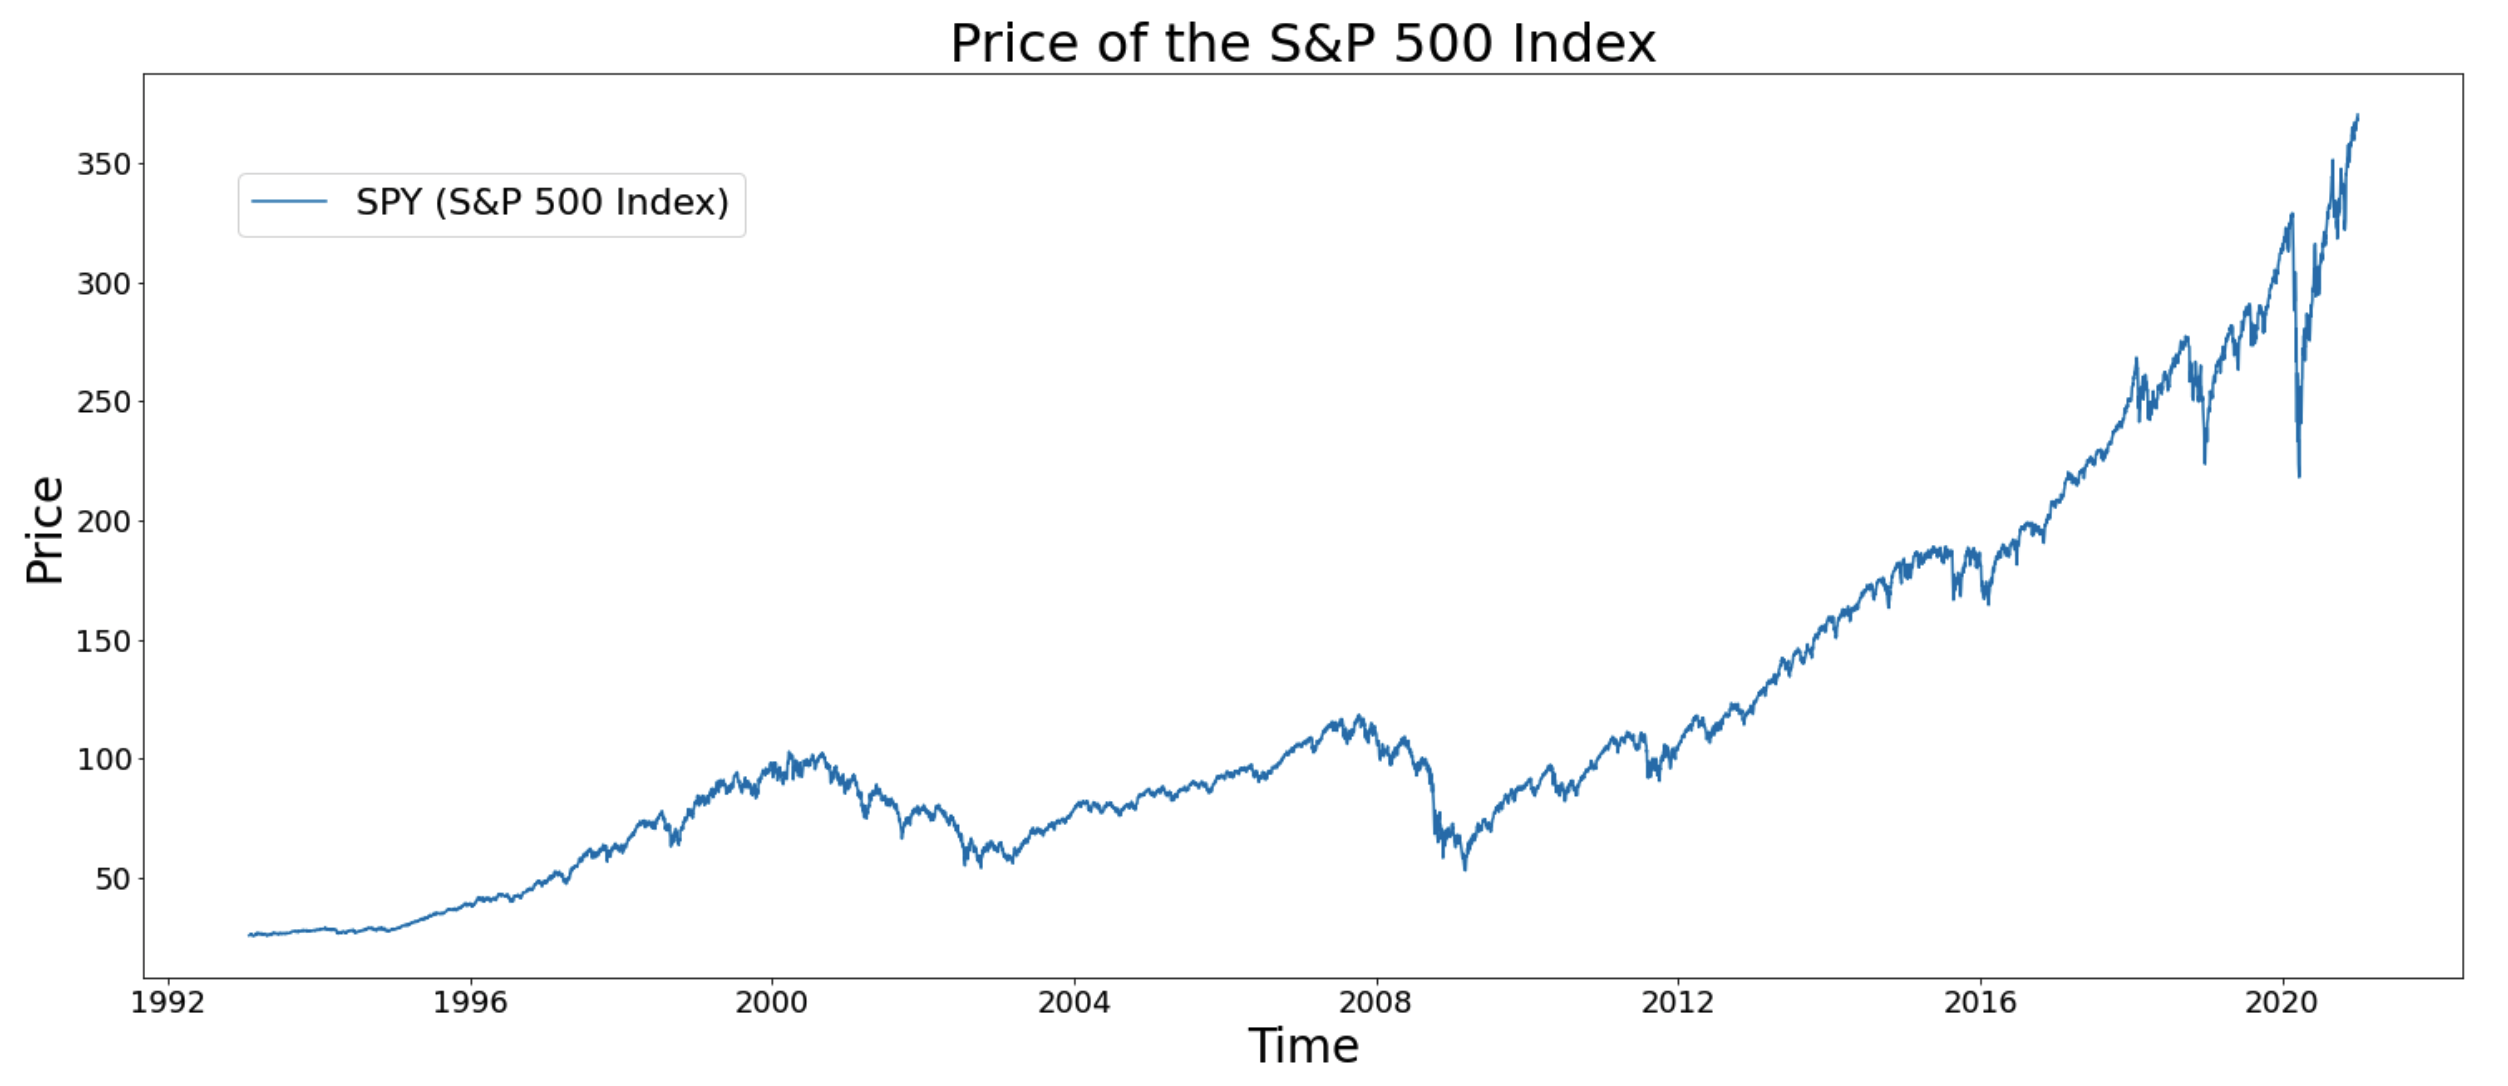
\includegraphics[width=\textwidth]{sp500price}
\caption{Price of the S\&P 500 index throughout for time period Jan. 29, 1993 to Dec. 31, 2020.}
\label{sp500price}
\end{figure}



\section{Models}

\subsection{Model 1: Simple Feed-Forward Neural Network}

We constructed a simple feed-forward neural network with 2 hidden layers (256 and 512 neurons), used LeRU as the activation function, and used MSE as our loss function.

Using stock data (price and volume), we built 15 features to feed into our neural network. The features are listed in Table \ref{fffeatures}.

\begin{table}[H]
\centering
\begin{tabular}{| c | l |} 
\hline
Number & Feature \\
\hline
1 & Stock Opening Price \\
2 & Stock Closing Price \\
3 & Stock Daily High Price \\
4 & Stock Daily Low Price \\
5 & Moving Average Convergence Divergence (MACD) \\
6 & Difference Between Stock Price and Bollinger Bands Low Range \\
7 & Difference Between Stock Price and Bollinger Bands High Range  \\
8 & Price Rate of Change (ROC) \\
9 & 12-Day Simple Moving Average (Fast SMA) \\
10 & 26-Day Simple Moving Average (Slow SMA) \\
11 & Difference Between Fast SMA and Slow SMA \\
12 & 12-Day Exponential Moving Average (Fast EMA) \\
13 & 26-Day Exponential Moving Average (Slow EMA) \\
14 & Difference Between Fast EMA and Slow EMA \\
15 & Relative Strength Index (RSI) \\
16 & Commodity Channel Index (CCI) \\
\hline
\end{tabular}
\caption{Table of all features used in our simple feed-forward neural network. (For simplicity, we will provide explanations of each of the features in the appendix in our final report)}
\label{fffeatures}
\end{table}

The output we would like to predict is the percentage of the stock price change 21 days in the future. We use this predicted output to construct buy / sell signals that will feed into our stock trading strategies.



\subsection{Model 2: Long Short-Term Memory Neural Network (LSTM)}

We constructed a long short-term memory neural network (LSTM) with 2 recurrent layers and 64 features in the hidden state. We used MSE as our loss function. An LSTM neural network is a recurrent neural network (RNN) that has feedback connections which make it a good model to run on time-series data (stock prices over time).

Our lookback period is 20 trading days. This means we will use the stock prices from the previous 20 days to predict the price of the next day. We tested with different lookback periods and concluded that 20 days yielded the best performance.



\section{Results}

We first establish baseline strategies before evaluating our models. We will use two simple strategies as our baseline: Buy \& Hold strategy and MACD strategy. Next we will develop trading strategies from the two neural network models described above.

\subsection{Strategies}

\subsubsection{Buy \& Hold Strategy}

The Buy \& Hold strategy is to use all original cash to buy the stock at the opening price at the start of the test period and sell all shares at the closing price at the end of the test period.


\subsubsection{MACD Strategy}

The MACD strategy is an established strategy that commonly yields better performance than the simple Buy \& Hold strategy. We will describe this strategy in detail below.

For the MACD strategy, we first plot the MACD line of a given stock, which is computed by subtracting the 26-day EMA (exponential moving average) from the 12-day EMA. Then we plot the MACD signal line, which is the stock's 9-day EMA. When the MACD line crosses over the MACD signal line, it triggers a buy signal. Conversely, when it crosses under, it triggers a sell signal.

For simplicity, we compute the MACD diff by subtracting the MACD signal from the MACD. The strategy will now trigger a buy signal if the MACD diff crosses over the $x=0$ line and trigger a sell signal if the MACD diff crosses under. See example in Figure \ref{macd}.

\begin{figure}[H]
\centering
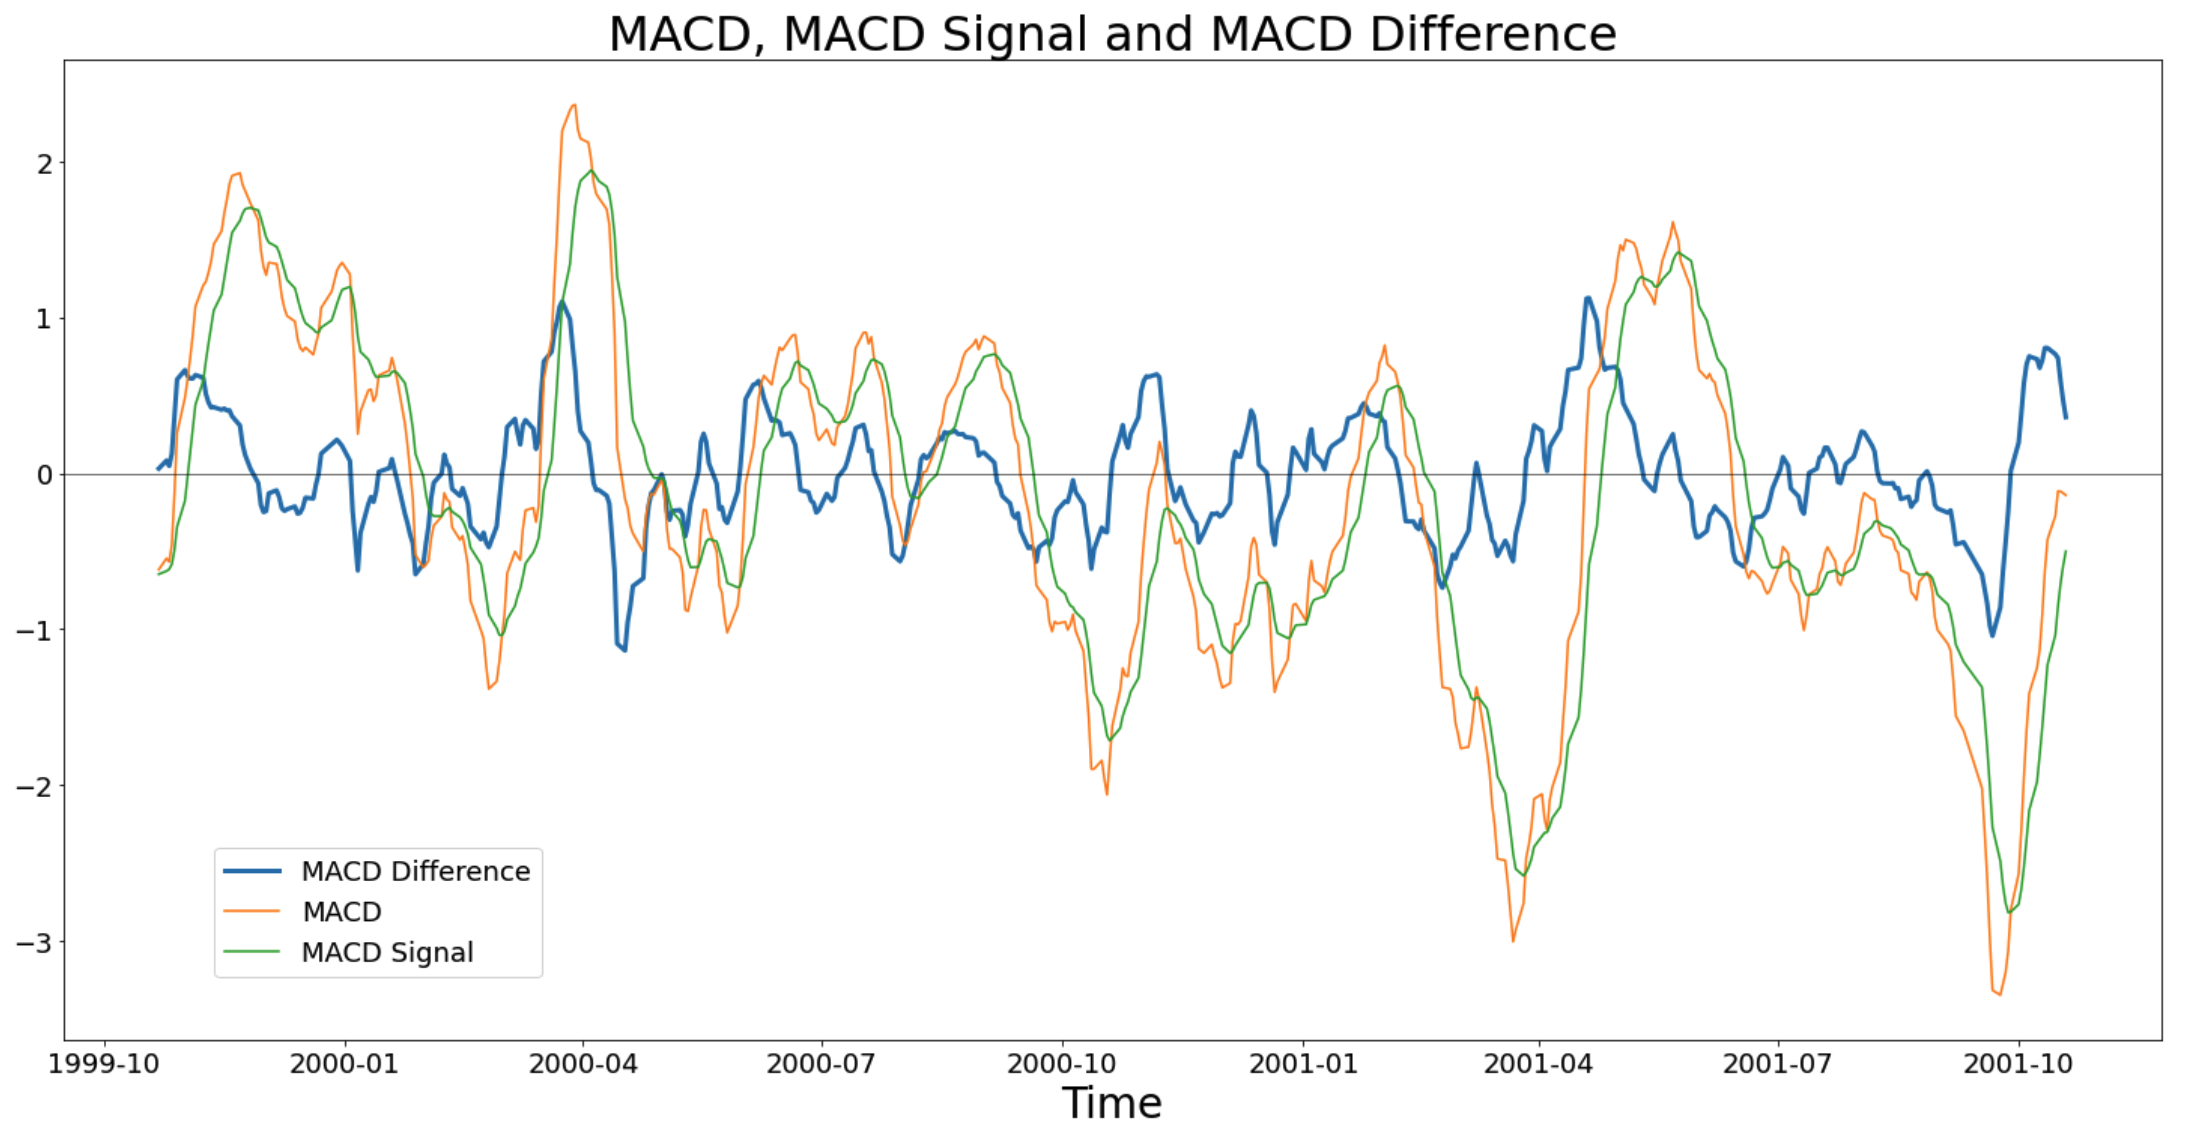
\includegraphics[width=\textwidth]{macd}
\caption{Sample MACD strategy with MACD, MACD signal, and MACD diff lines. Buy signals are triggered when MACD diff line crosses over the zero line and sell signals are triggered when MACD diff line crosses under the zero line.}
\label{macd}
\end{figure}


\subsubsection{FF Strategy}

The FF strategy is developed from our simple feed-forward neural network model above. We trained our model using training data and used the model to develop trading strategies. Then we ran the strategy on our test data to evaluate its performance.

The model predicted the 21-day price change in the future. If the price change is $> +0.5\%$, then we trigger a buy signal and if the change is $< -0.5\%$, we trgger a sell signal, otherwise we hold.


\subsubsection{LSTM Strategy}

The LSTM strategy is developed from our LSTM above. We use our LSTM model to predict future stock prices based on the historical stock prices of a lookback period (21 days). We trained our model on the training set and plot the predicted stock prices against the actual stock prices in Figure \ref{lstmtrain}.

\begin{figure}[H]
\centering
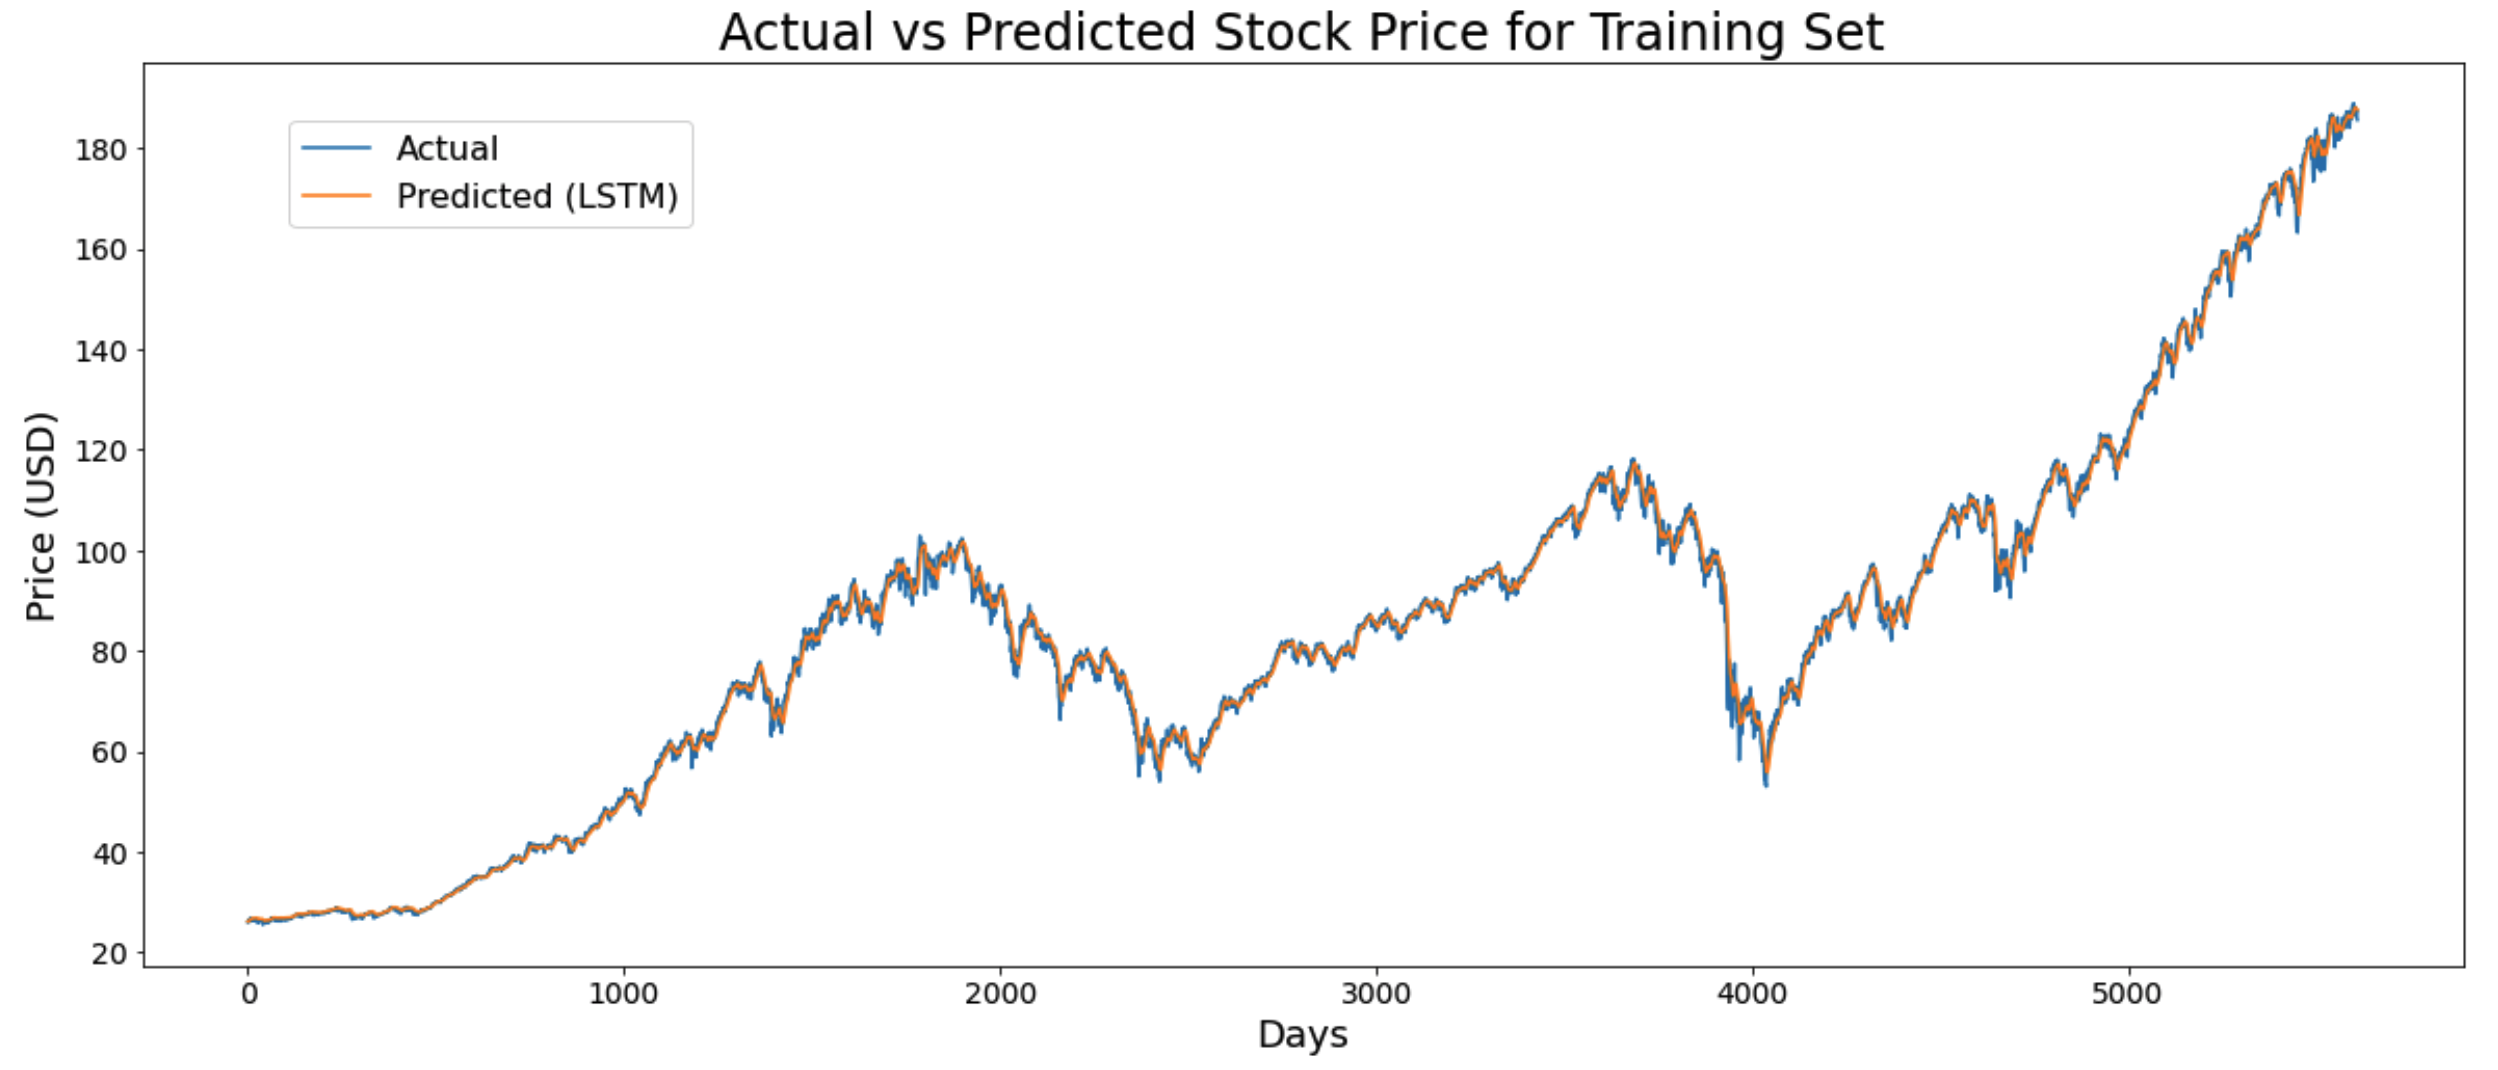
\includegraphics[width=\textwidth]{lstm-train}
\caption{Predicted stock price vs actual stock price for the training set.}
\label{lstmtrain}
\end{figure}


Then we run our trained model on the test set and plot the predicted stock prices against the actual stock prices in Figure \ref{lstmtest}.

\begin{figure}[H]
\centering
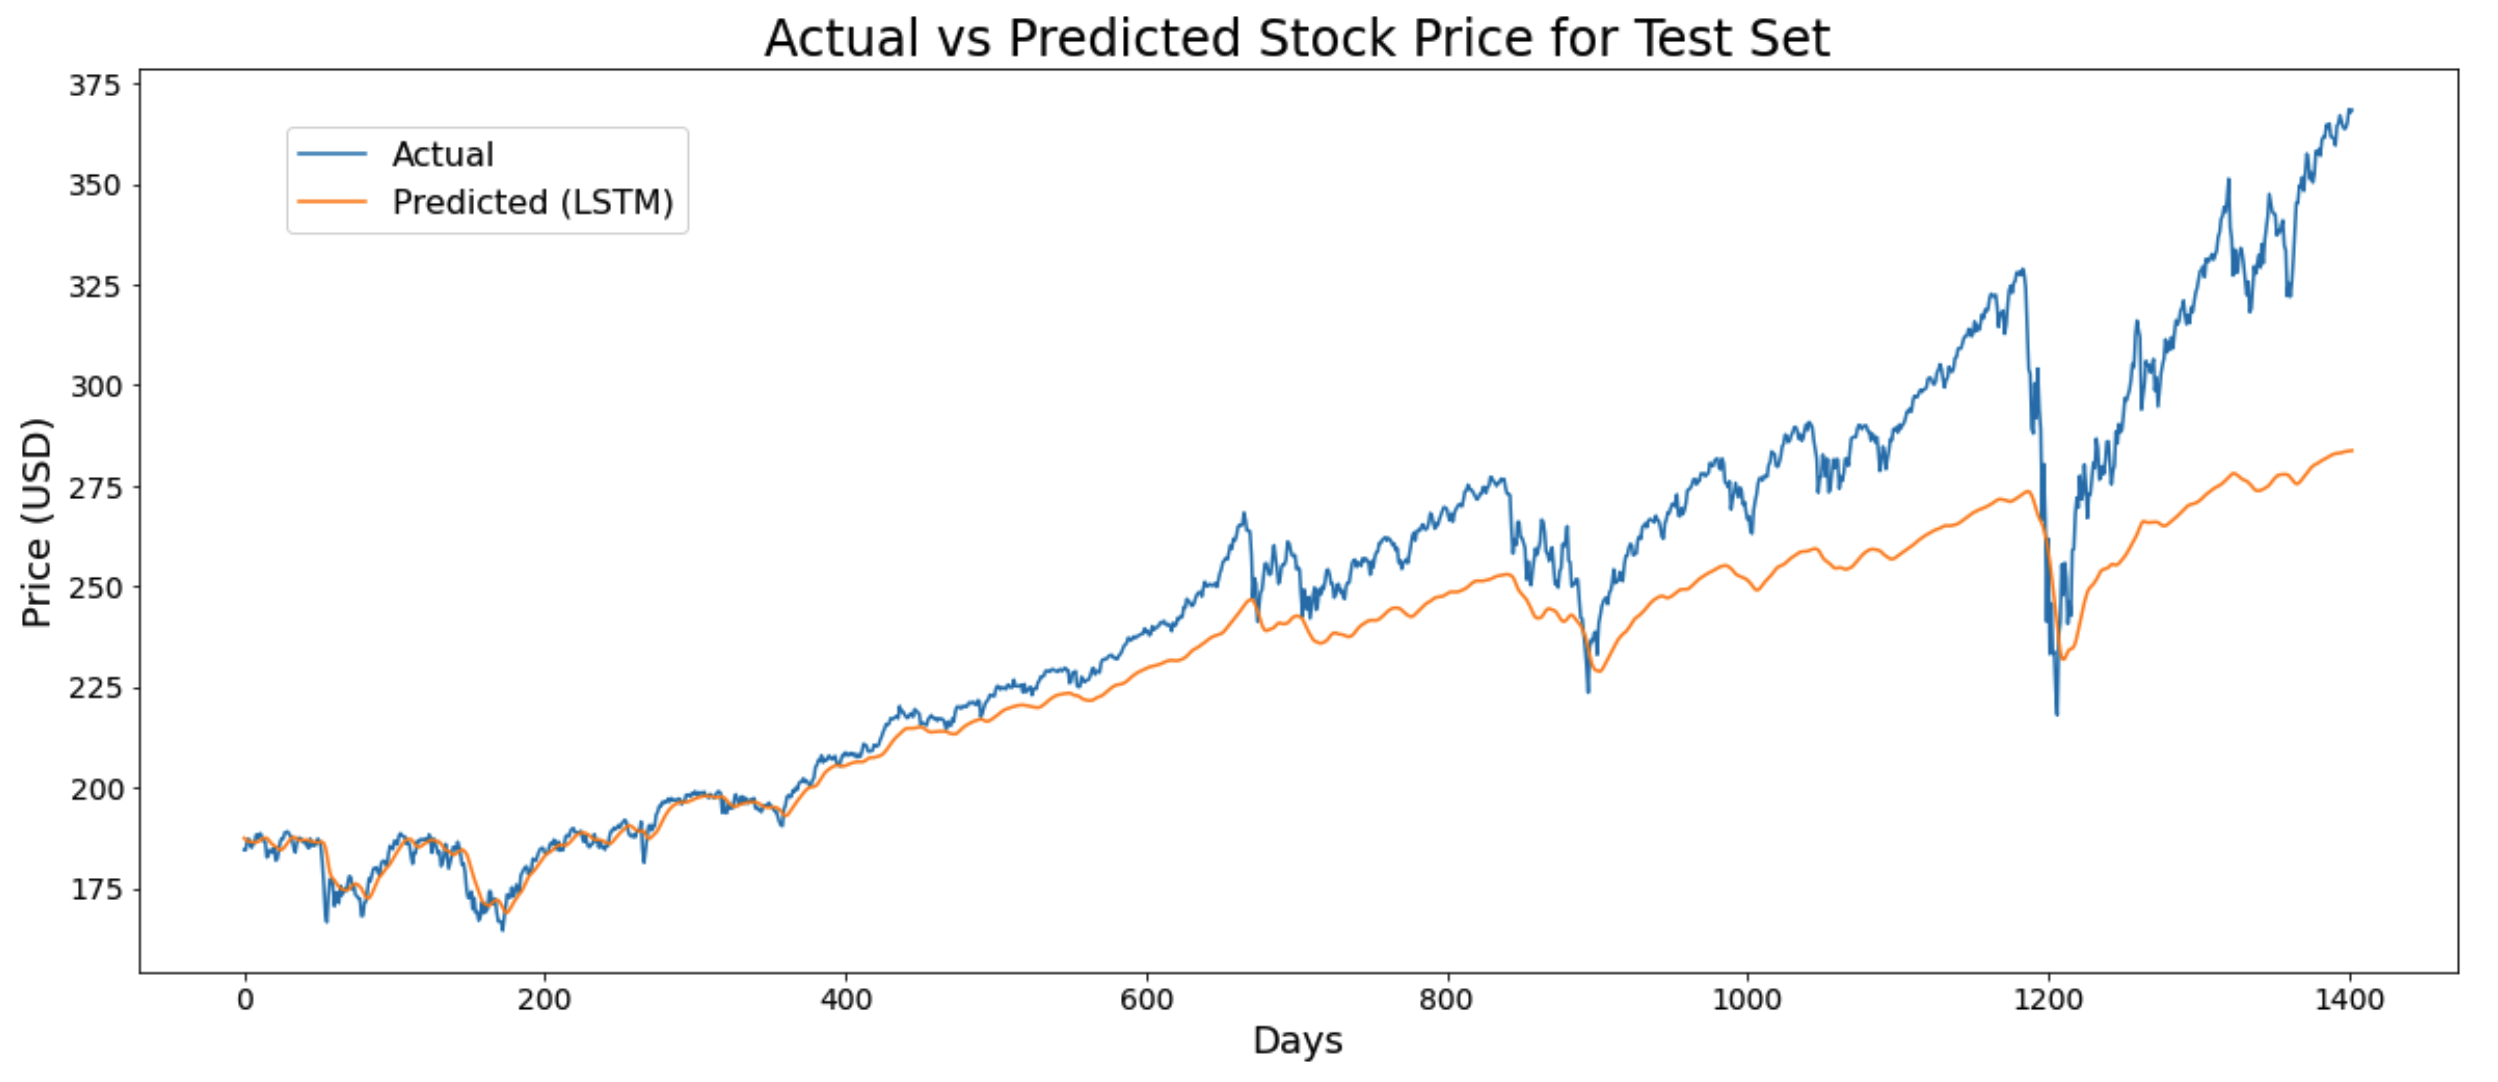
\includegraphics[width=\textwidth]{lstm-test}
\caption{Predicted stock price vs actual stock price for the test set.}
\label{lstmtest}
\end{figure}

From Figure \ref{lstmtest}, we can see that even though the price values differ, the general trend of the price movement matches. We use this information to develop a strategy by triggering a buy signal when the predicted price is greater than the current price and a sell signal when the predicted price is lower than the current price.


\subsection{Evaluation}

To evaluate our strategies, we developed a strategy evaluator. This evaluator starts out with \$100,000 cash and will buy the maximum possible shares if a buy signal is triggered and will sell all shares when a sell signal is triggered. Because we generate a buy / sell signal after trading hours, we use the opening price of the next day for executing the buy / sell signal.

At the end of the test period, the evaluator adds up the value of the remaining cash and the current value of the shares (by using the closing price of the final day).

Using this evaluation strategy, we can test the performance of all 4 strategies listed above.

\begin{figure}[H]
\centering
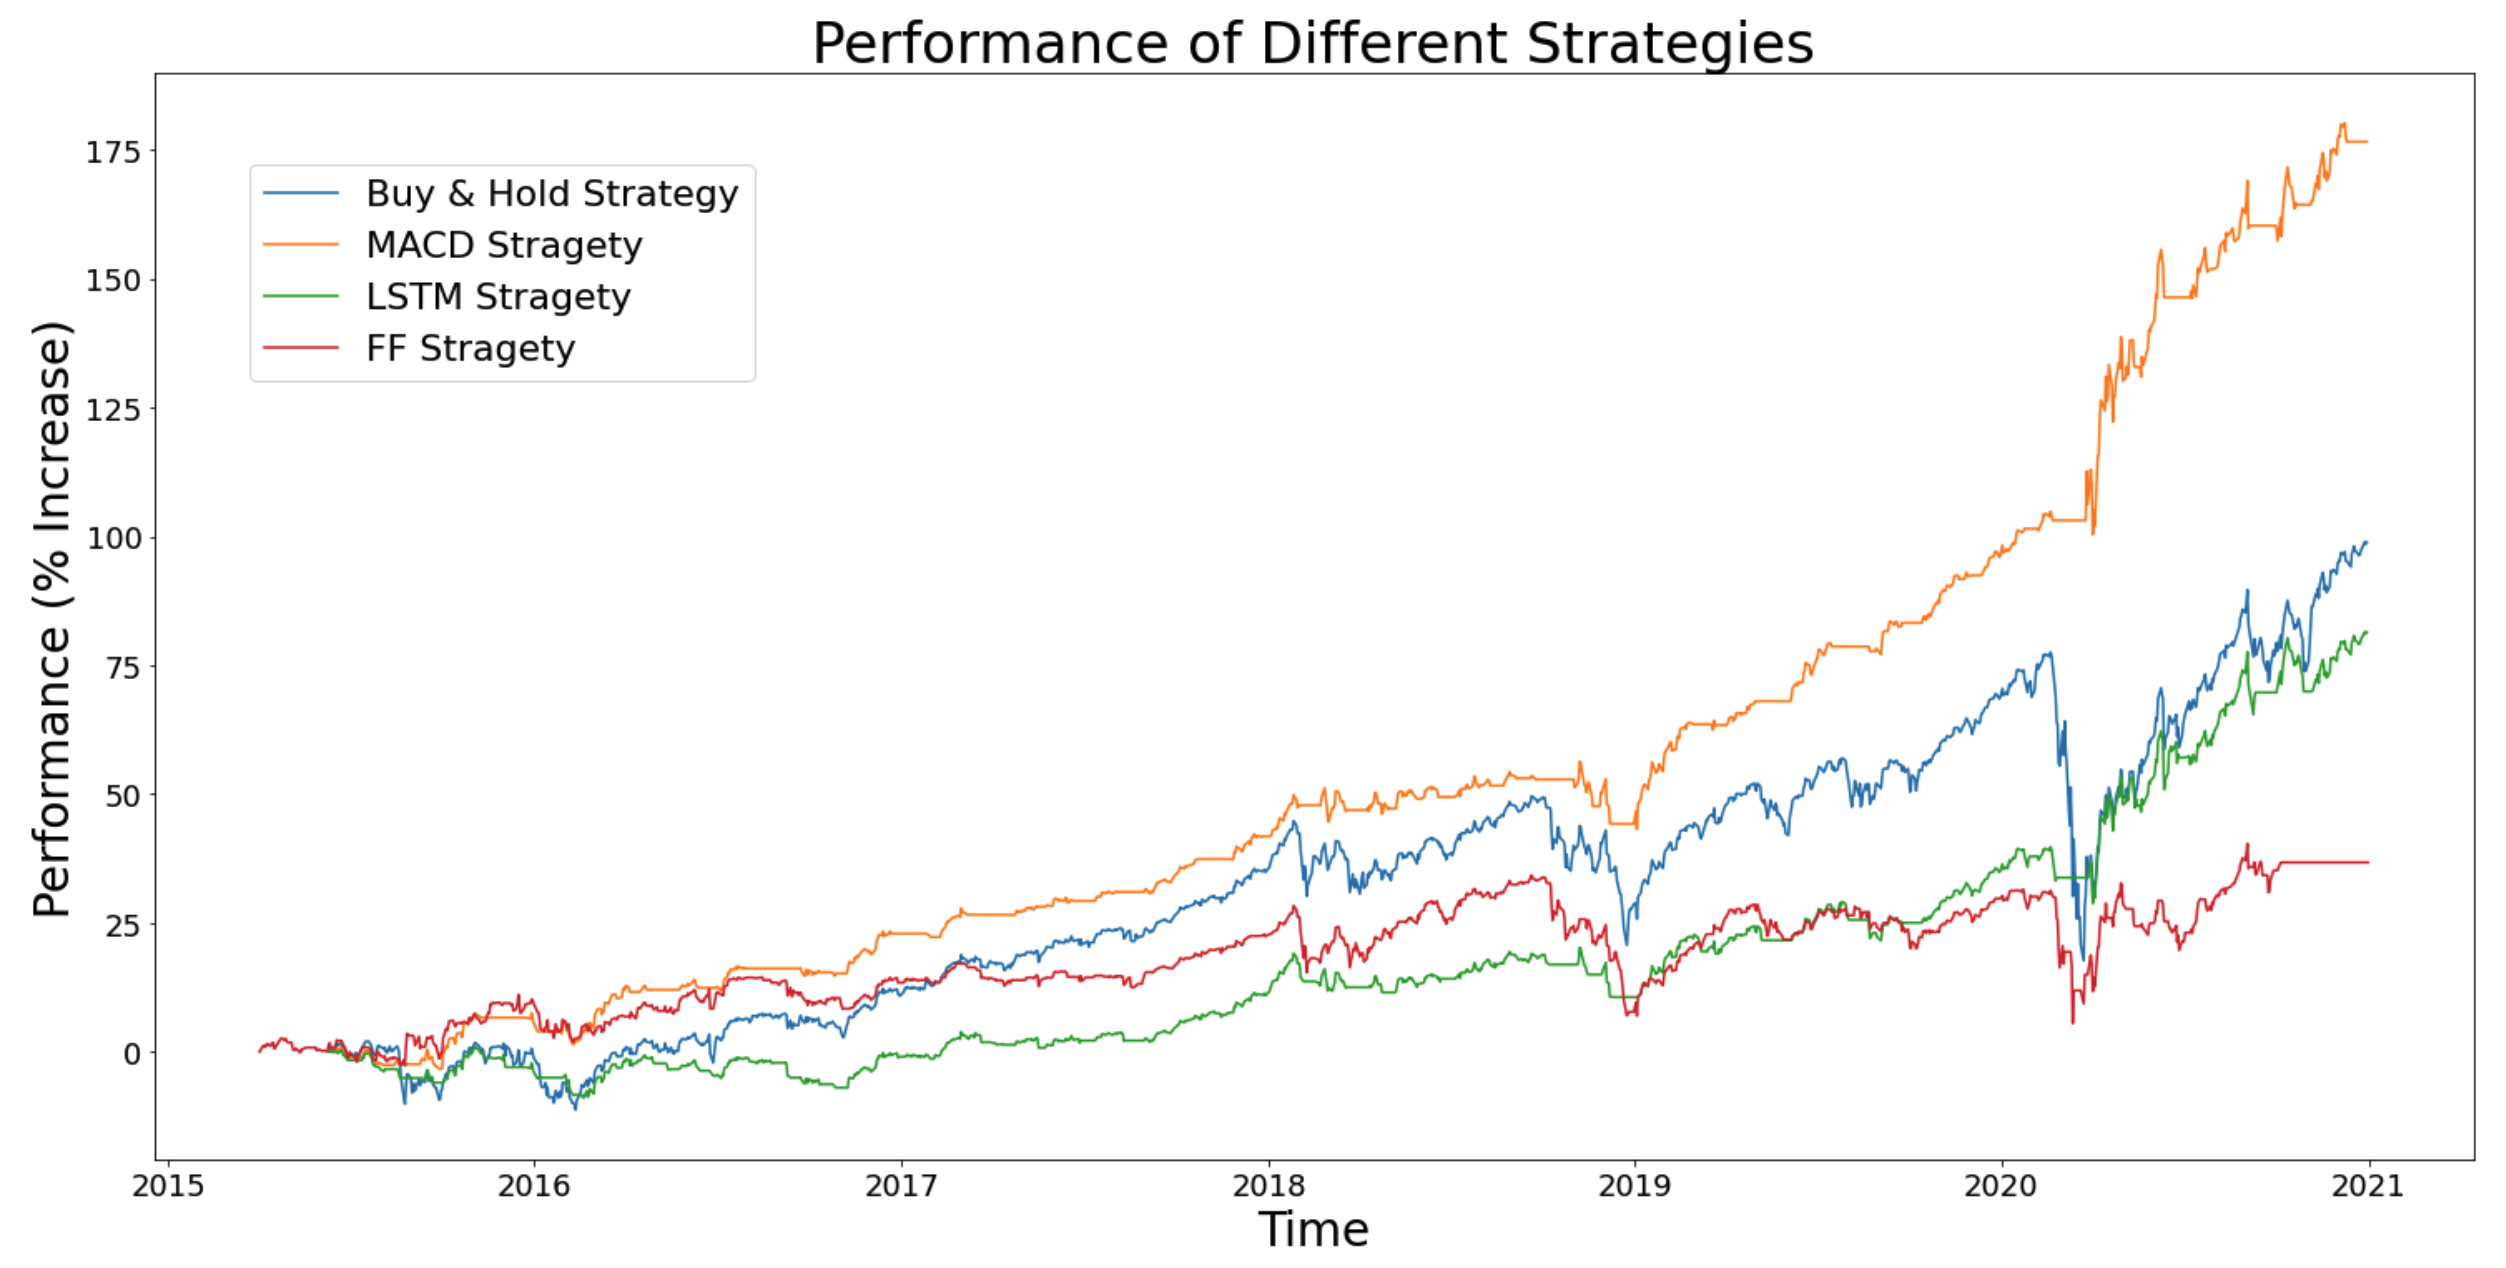
\includegraphics[width=\textwidth]{perf}
\caption{Performance curves of 4 trading strategies.}
\label{perf}
\end{figure}

\begin{table}[H]
\centering
\begin{tabular}{| l | l |} 
\hline
Strategy & Performance \\
\hline
Buy \& Hold Strategy & 98.8370\% \\
MACD Strategy & 176.5809\% \\
LSTM Strategy & 81.4012\% \\
FF Strategy & 36.7426\% \\
\hline
\end{tabular}
\caption{Performance of 4 trading strategies given by the percent increase in portfolio value.}
\label{perftable}
\end{table}

From Figure \ref{perf} and Table \ref{perftable}, we can see that the MACD strategy performs best, followed by the Buy \& Hold strategy and the LSTM strategy. The FF strategy performs worst.


\section{Analysis and Future Work}

Our preliminary results show that our neural network strategies perform worse than the already established strategies (Buy \& Hold and MACD). We will analyze their performance and future work below.

The FF strategy uses technical indicators to predict future stock prices. Although this may seem like a compelling case, it doesn't work well because the stock market behaves randomly. It is hard to use technical indicators from a single day to predict future prices.

On the other hand, the stock market does indeed follow some trends. This allows use to use the characteristics of LSTM neural networks to ``remember" some historical data and use this ``memory" to predict future prices.

As we can see from the analsis above, we can see that the LSTM strategy is only slightly worse than the Buy \& Hold strategy. Currently we are only using the closing stock prices of the previous 21 days to predict the price of the next day. We can try to improve our existing model by adding more features to the LSTM model. We can also try to train a more complex model than our current one.

Currently we only evaluated our strategies on the S\&P 500 index. For future work, we will also try to evaluate our strategies on other indices such as the Nasdaq index and the Dow Jones Industrial Average. Furthermore, we will also try to apply our strategies on some individual stocks and evaluate performance. This important to see whether our strategies work more generally.


\end{document}
